%----------------------------------------------------------------------------
\chapter{Android alkalmazás beszélőfelismerésre}
%----------------------------------------------------------------------------

A következő fejezetben bemutatom egy általam a beszélőfelismerés szemléltetésére készített android alkalmazás fő elemeit és működését, a kapcsolódó technológiákat és implementációs részleteket. Az alkalmazásban konkrét beszélőfelismerésre készített neurális hálózatokat használok fel. A cél nem egy új beszélőfelismerő modell készítése volt, hanem az eddigiek felhasználásával egy működő alkalmazás létrehozása.
\newline
\newline
Az alkalmazás kliens-szerver architektúrájú. Az android kliens segítségével a felhasználó regisztrálhat a rendszerbe névvel és hanggal, majd az azonosítás opció megnyomásával hangmintát adva az alkalmazás eldönti, hogy regisztrálva van-e, és ha igen, akkor visszaadja az illető nevét.

\section{Modell predikció a felhőben vagy lokálisan?} \label{cloud_or_local}


A szervernek tárolnia kell a felhasználóktól származó hangmintákat és a felhasználó azonosítás folyamata közben összehasonlítani őket. Az összehasonlítást egy sziámi neurális hálózat végzi. Az alkalmazás felépítését tekintve a legfontosabb kérdés, hogy ezt az összehasonlítást központilag egy felhőben a szerver, vagy a kliens oldali alkalmazás végezze. Mivel a modell végzi a predikciót, ettől a döntéstől függően azt a szerveren vagy a kliens eszközökön kell tárolni. Mindkét architektúrának vannak előnyei és hátrányai is.
\newline
\newline
Mivel esetünkben az alkalmazás kész, előre tanított modelleket használ, nincs szükség a modellek tanítására. Ennek ellenére ha a jövőben saját modellt szeretnénk használni felmerül a kérdés, hogy hol tanítsuk azt~\cite{cloud_or_local}.

\begin{itemize}
	\item A felhőben hosztolt gépi tanulási szolgáltatások általában saját modelleket használnak. Mi a saját adatainkat átadjuk és a szolgáltatás gondoskodik a modell tanításáról. Ezután a predikciót egy API-n keresztül végezhetjük el. Figyelni kell arra, hogy ebben az esetben nem mindig miénk a modell. Ha nincs lehetőség tanítás után a modell letöltésére, akkor a predikció mindenképp a felhőben marad. Másrészről a magas szintű szolgáltatások kezelése könnyebb, nem kell érteni a neurális hálózatok tanításához, de nem elég flexibilisek. Általában nem változtathatunk a modellen és az API-n sem.
	
	\item A felhőben taníthatjuk a modellünket az erre készített szolgáltatások nélkül is nagyobb hozzáértést feltételezve. Ekkor megválaszthatjuk a modell típusát és a technológiákat (Tensorflow, Pytorch, stb.) és teljes mértékben miénk a modell és az irányítás. A lokális tanítással szemben további előny, hogy az erőforrásokat rugalmasan fel-le skálázhatjuk.
	
	\item Lokálisan is taníthatjuk a modellt. Ez főleg akkor éri meg, ha van elég erőforrásunk hozzá vagy a modell mérete nem indokolja több erőforrás használatát. Nagyobb modellek esetében a tanítási idő hosszú. Az árakat és az időt mérlegelve dönteni kell, hogy a lehetőségek közül melyiket indokolt választani.
\end{itemize}
\ \\
Ha már rendelkezünk egy működő modellel, akkor el kell döntenünk, hogy a predikciót a felhőben vagy lokálisan az eszközön végezzük.

\begin{itemize}
	\item A hálózati kapcsolatot tekintve ha a predikciót lokálisan végezzük, nincs szükség internetkapcsolatra, predikció a készüléken történik. Ellenkező esetben a kliens interneten keresztül kérést küldd a szervernek, ami elvégzi a predikciót és visszaküldi a választ.
	\item A modellt felhőben a szerveren tárolni biztonságosabb. Lokális predikció esetén a modellt a készüléken tároljuk. Ilyenkor gondoskodni kell a biztonságáról, hogy ne lehessen visszafejteni azt (reverse engineering).
	\item A predikció sebessége is meghatározó szempont. Ha lokálisan, a mobiltelefon hajtja végre, a felhőhöz képest kisebb erőforrással gazdálkodunk, ami miatt lassabb lesz a számítás. Viszont ha a felhőben végezzük, a kommunikációs overhead hozzáadódik a válaszhoz. Le kell mérni, hogy a kliens-szerver kommunikáció késleltetése mekkora az erőforráskülönbségből származó számítási időkhöz képest.
	\item Az alkalmazás architektúráját tekintve ha a modell és a predikció a szerveren történik, bármikor frissíthetjük, finomhangolhatjuk a modellt és ehhez nem kell a felhasználóknak frissítéseket letölteniük. Nincs szükség szinkronizációra. Az alkalmazás elosztott, elkülönült backend és frontend részekből áll, amelyek egy interfészen keresztül kommunikálnak, így ezek a komponensek lecserélhetők, csak az interfészt kell implementálniuk (API).
	\item Felhőbeli erőforrásokat használva az árat is figyelembe kell venni. Minél több felhasználó használ egy alkalmazást és amennyiben a számítás központilag a felhőben történik, annál több erőforrásra van szükség. Nagy előnye a készüléken végzett predikciónak, hogy jól skálázódik. Több felhasználó esetén nincs szükség több erőforrásra.
\end{itemize}
\ \\
Jelen alkalmazás egy beszélőfelismerő szoftvert szemléltet, amelyet a valóságban vállalatok üzemeltetnek beléptető kapuval biometrikus azonosításra használva. Központi szerverre szükség van a regisztrált felhasználók adatainak biztonságos tárolása és a könnyű szinkronizáció miatt. Ha feltesszük, hogy a beléptető rendszert nem több mint tízezer ember azonosítására használják és a belépés szekvenciálisan történik, óriási erőforrásokat sem kell használni, mert a szerver egy időben legfeljebb a beléptető kapuk száma szerinti számítást kell végezzen, ami korlátos. Ezeket figyelembe véve úgy döntöttem, hogy a modell tárolása és a predikció szerveren fog történni.

\section{Alkalmazás architektúra és általános működés}

Mivel az alkalmazás tárolja a regisztrált felhasználók hangmintáit és a modellt; a biztonság, a könnyű központi adminisztráció és a tény, hogy nincs szükség szinkronizációra mind megerősíti a kliens-szerver architektúra szükségességét és előnyeit, így peer-to-peer megoldás fel sem merült.

\begin{figure}[H]
	\centering
	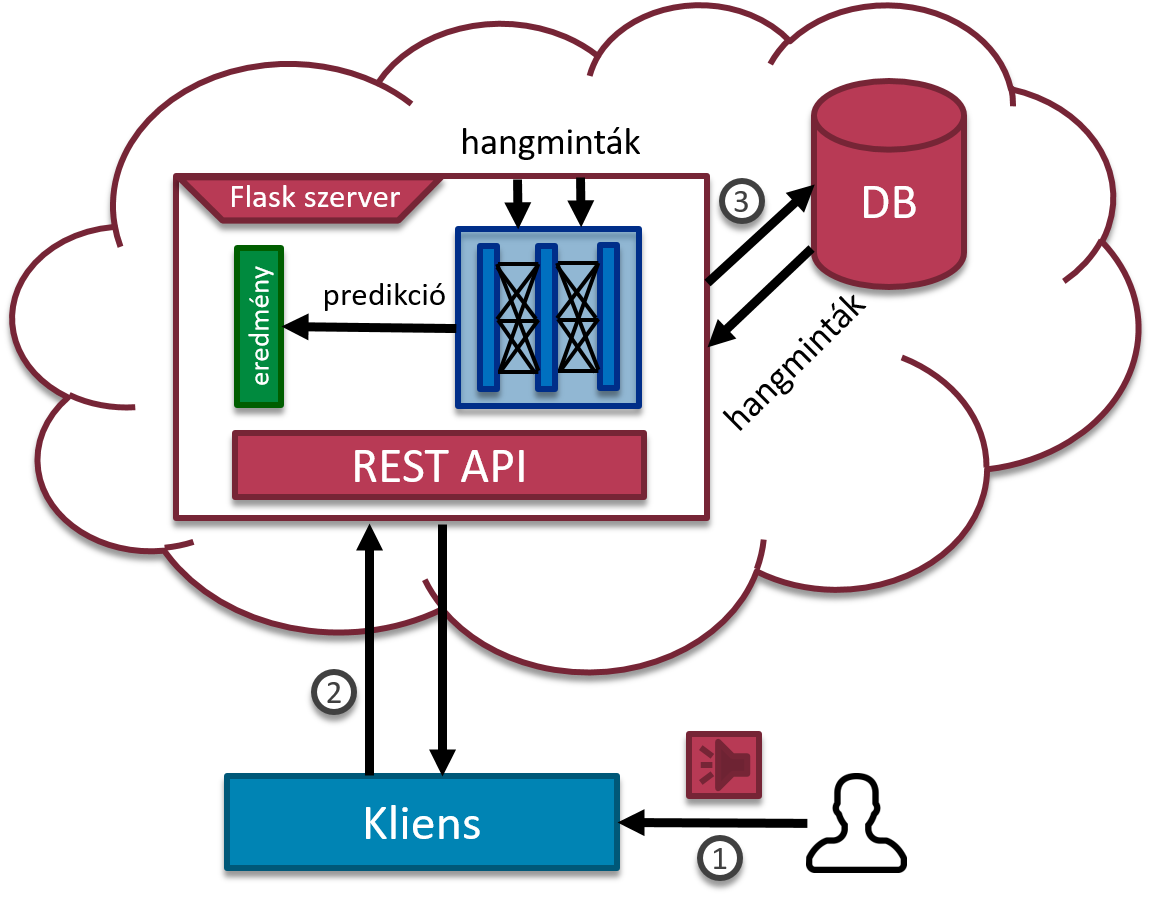
\includegraphics[width=100mm, keepaspectratio]{figures/app-register.png}
	\caption{Beszélőfelismerő alkalmazás: Regisztrációs fázis.}
	\label{fig:app-register}
\end{figure}
\ \\
A \ref{fig:app-register} ábrán látható kliens a felhőben futó szerverrel egy REST API-n keresztül kommunikál. A kliens segítségével a felhasználó regisztrál a rendszerbe, ezután azonosíthatja magát. A regisztrációs fázis működése a következő:

\begin{enumerate}
	\item A kliens alkalmazás rögzíti a felhasználó hangját és nevét.
	\item A kliens a hangmintát és a nevet elküldi a szervernek a REST API-n keresztül.
	\item A szerver előfeldolgozza a hangfájlt, a modell segítségével hangvektort készít belőle és menti az adatbázisba. 
\end{enumerate}
\ \\
Miután a felhasználók regisztráltak, az alkalmazás a hangjuk alapján azonosítani tudja őket. Az azonosítási fázis lépéseit a \ref{fig:app-identify} ábra mutatja.

\begin{figure}[!ht]
	\centering
	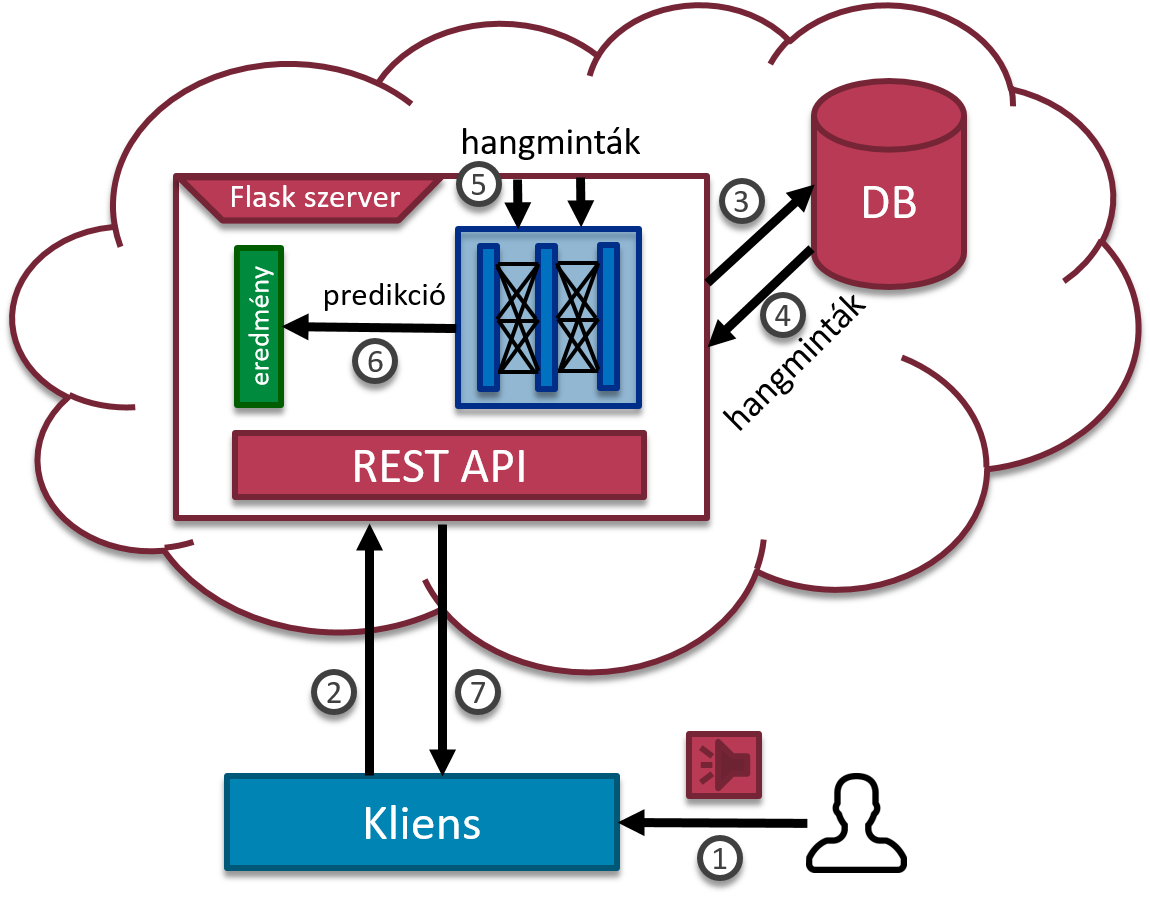
\includegraphics[width=100mm, keepaspectratio]{figures/app-identify.png}
	\caption{Beszélőfelismerő alkalmazás: Regisztrációs fázis.}
	\label{fig:app-identify}
\end{figure}

\begin{enumerate}
	\item A kliens rögzíti az azonosítani kívánt felhasználó hangját.
	\item A hangmintát továbbítja a szervernek.
	\item A szerveren futó alkalmazás a hangfájlt előfeldolgozza és hangvektort készít belőle.
	\item A szerver kiszámolja a hangminták közötti hasonlósági pontokat. A minimálishoz tartozó felhasználó nevét elküldi a kliensnek.
\end{enumerate}

\subsection{Biztonsági funkciók}

Azt is figyelembe kell venni, hogy azonosításkor a szerver a minimális vektortávolsághoz tartozó névvel tér vissza. Ez azt jelenti, hogy ha egy regisztrált felhasználó van a rendszerben,
bárki képes lenne belépni a regisztrált felhasználó nevében, hiszen csak egy távolság van, ami minimális. Ennek elkerülésére további biztonsági funkciókkal kell kiegészíteni az alkalmazást.
\newline
\newline
Meg kell határozni egy biztonsági küszöböt a vektorok távolságára - azaz ha nem elég hasonlóak, egyéb autentikációs mechanizmusra lesz szükség. Ennek megfelelően a szervert
kiegészítettem egy biztonsági küszöbbel, amit ha azonosításkor a vektortávolság meghalad, jelszó alapú azonosítást kér a felhasználótól. A biztonsági funkcióval kiegészített
működés abban az esetben, ha a biztonsági küszöböt meghaladja az alkalmazás a \ref{fig:app-with-security} ábrán látható. A regisztrációs fázis annyiban tér el az előzőtől, hogy a felhasználó egy jelszót is megad a neve mellett, amit
a szerver eltárol.

\begin{figure}[H]
	\centering
	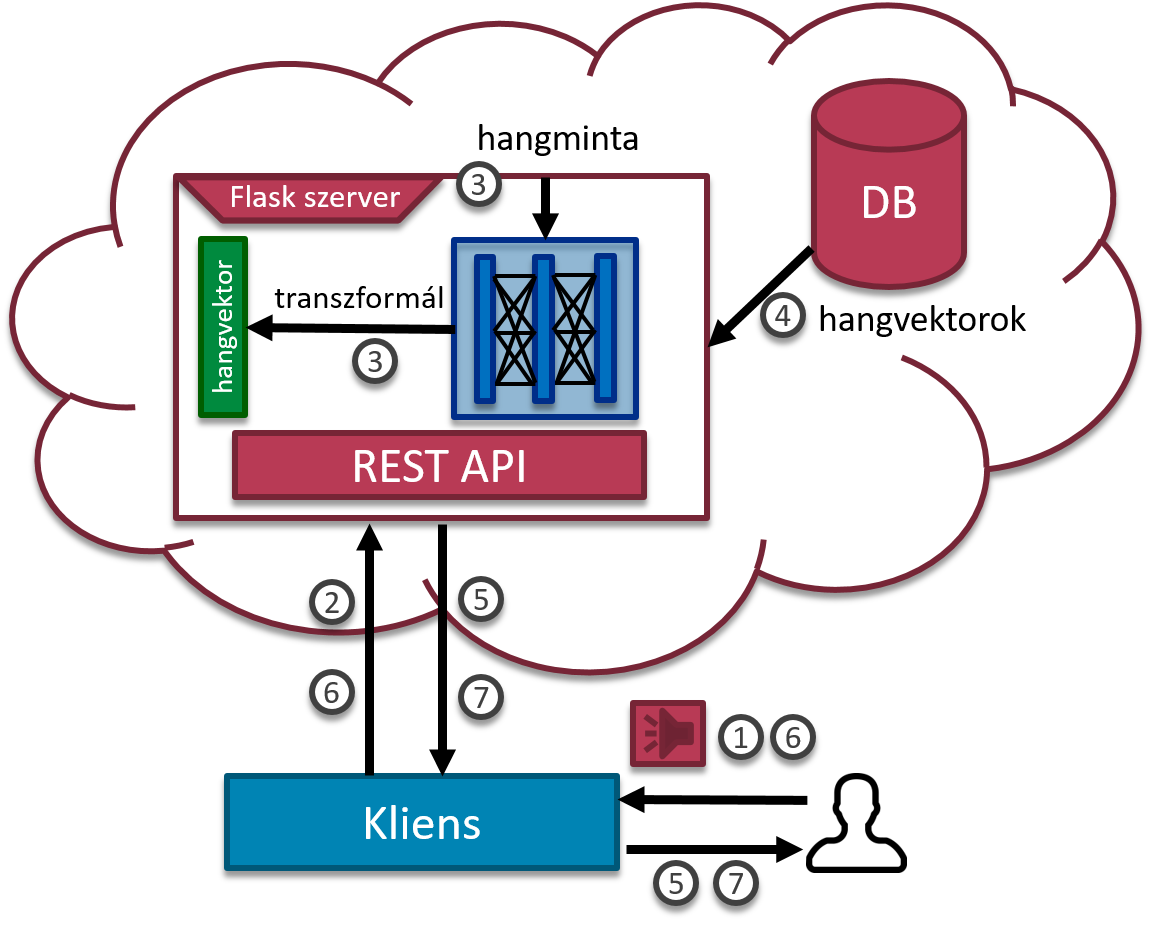
\includegraphics[width=100mm, keepaspectratio]{figures/app-with-security.png}
	\caption{Beszélőfelismerő alkalmazás: Azonosítás jelszó alapú autentikációval.}
	\label{fig:app-with-security}
\end{figure}
\newpage
\begin{enumerate}
	\item A kliens rögzíti az azonosítani kívánt felhasználó hangját.
	\item A hangmintát továbbítja a szervernek.
	\item A szerveren futó alkalmazás a hangfájlt előfeldolgozza és hangvektort készít belőle.
	\item A szerver összehasonlítja a hangvektort a korábban eltároltakkal és kiszámol egy hasonlósági pontot vagy vektortávolságot.
	\item A pontszám meghaladja a biztonsági küszöböt, ezért kliensnek felszólítást küld, hogy jelszó alapú autentikációt kér.
	\item A kliens megadja a saját jelszavát, amivel  korábban regisztrált és elküldi a szervernek.
	\item A szerver ellenőrzi, hogy a megadott jelszó valóban az azonosítani kívánt felhasználóhoz tartozik-e. Amennyiben igen, visszaküldi az azonosított felhasználó nevét,
	egyébként jelzi, hogy az autentikáció sikertelen volt.
\end{enumerate}

\subsection{Vektorok átlagolása}

A vektorok átlagolása egy opcionális funkció. A szerver oldali alkalmazás minden sikeres azonosítás után átlagolja a tárolt vektort az aktuálisan azonosítottal. Azonosításkor ha a hasonlósági pontszám
a biztonsági küszöb alatt van, az átlagolás minden további nélkül megtörténik.
Amennyiben a minimális vektortávolság nem üti meg a küszöbszintet az alkalmazás az aktuális vektort ideiglenesen eltárolja. Ezután ha a felhasználó sikeresen autentikál jelszóval, a vektort átlagolja a korábbival majd törli, egyébként csak törli azt.


\subsection{Konfiguráció}

A szerver oldali alkalmazás képes többféle hasonlósági pontot számolni
a vektorok között. A jelenlegi implementáció a következő hasonlósági pontokat támogatja $v_1=(x_1, x_2, \dots)$ és $v_2=(y_1, y_2, \dots)$.

\begin{itemize}
	\item Euklideszi-távolság: $$d_{euc}(v_1, v_2) = \left (\sum_{i=1}^{n} x_i - y_i \right) ^\frac{1}{2}$$
	\item Koszinusz-távolság: $$d_{cos}(v_1, v_2) = \frac{v_1 \cdot v_2}{\left\lVert v_1 \right\rVert \cdot \left\lVert v_2 \right\rVert} = \frac{\sum_{i=1}^{n} x_i \cdot y_i}{\sqrt{\sum_{i=1}^{n} x_i^2} \cdot \sqrt{\sum_{i=1}^{n} y_i^2}}$$
\end{itemize}
\ \\
Konfigurálható továbbá a biztonsági küszöbszám is. Ez annak az értéke, amelyet
ha a hasonlósági pontszám meghalad, a szerver jelszó alapú autentikációs kérést küld a kliens fele.

\section{Implementáció}

\subsection{Kliens alkalmazás}

Ebben a fejezetben részletesen bemutatom az alkalmazás fő komponenseinek működését, felépítését és a fejlesztőkörnyezet részeit.

\subsubsection{Projekt felépítése}

Az Android Studios projekt főbb elemei a következők:

\begin{itemize}
	\item \emph{AndroidManifest.xml}: Engedélyek és activityk deklarálása.
	\item \emph{java}: Activitykhez tartozó és egyéb java osztályok.
	\item \emph{res/layout}: A felhasználói felülethez tartozó xml leírók.
	\item \emph{build.gradle}: Gradle modul konfiguráció és dependenciák módosítására.
\end{itemize}

\subsubsection{Engedélyek}

Bizonyos műveletek elvégzéséhez az Android operációs rendszeren engedélyek szükségesek. Az engedélyek a művelet típusától függően \emph{normál} vagy \emph{veszélyes} osztályba tartoznak. Ha az alkalmazás olyan műveletet akar végrehajtani, amihez engedély szükséges, azt deklarálni kell az android projekt manifest fájljában.
\newline
\newline
A \emph{normál} engedélyeket az operációs rendszer ezután automatikusan biztosítja, míg a \emph{veszélyesekhez} a felhasználó engedélyét kéri. Korábbi android verziókban az engedélyek megadási az alkalmazás telepítésekor történt, de később ez megváltozott. A minimum Android 6.0-át (23-as API szint) használó készülékeken a felhasználó már nem telepítéskor, hanem futási időben kell megadja az engedélyeket. Egy felugró ablak listázza, hogy az alkalmazás milyen engedélyeket kér, ezután választhat, hogy melyeket adja meg neki.
\newline
\newline
A beszélőfelismerő alkalmazás a következő engedélyeket használja:

\begin{itemize}
	\item RECORD\_AUDIO: A mikrofon használata hangfelvételhez.
	\item READ\_EXTERNAL\_STORAGE: A külső tárhely olvasásához.
	\item WRITE\_EXTERNAL\_STORAGE: A külső tárhely írásához.
	\item INTERNET: Internetelérés hálózati kommunikációhoz.
\end{itemize}

\subsubsection{Tárhely}

Az alkalmazás a felhasználótól vett hangmintát \emph{wav} formátumban tárolja el. A \emph{wav} egy tömörítetlen audioformátum és mivel később hangmintából jellemzőkinyerés történik, így nem veszíthetünk információt a jellemzőkről a tömörítés miatt. Később bemutatom, hogy a tömörített audioállományok milyen hatással vannak a modell teljesítményére.
\newline
\newline
Az Android beépített \emph{MediaRecorder} osztálya a \emph{wav} formátumot nem támogatja és nincs erre készült más beépített Java osztály sem, ezért egy erre készített kódot használtam fel Selvaline blogjáról. Selvaline \emph{WavRecorder} osztálya az általunk beállított paraméterekkel (csatorna, mintavételi frekvencia, stb.) felveszi a hangot és egy \emph{wav} fájlban tárolja azt.
\newline
\newline
Az Android operációs rendszeren használhatunk külső és belső tárhelyet. A belső tárhely előnye, hogy a fájlokhoz csak az alkalmazás fér hozzá és annak eltávolításakor a hozzá kapcsolódó fájlok is törlődnek. A külső tárhely előnye esetünkben, hogy könnyű mountolni. Ha a készüléket USB-vel számítógéphez csatlakoztatjuk, a külső tárhelyen lévő fájlokat böngészhetjük. Ez a hangfájl tesztelése miatt célszerű választás volt. 



\subsubsection{Felhasználói felület}

 A felhasználói felület három részből áll és minden felülethez egy-egy \emph{Activity} osztály tartozik. A fő felületen választhat a felhasználó a regisztráció és az azonosítás között. A fő felületen az \emph{Enroll} gombot megnyomva a regisztrációs, illetve ehhez hasonlóan az \emph{Identify} opcióval az azonosító felületre ugorhatunk.


\begin{figure}[!ht]
	\centering
	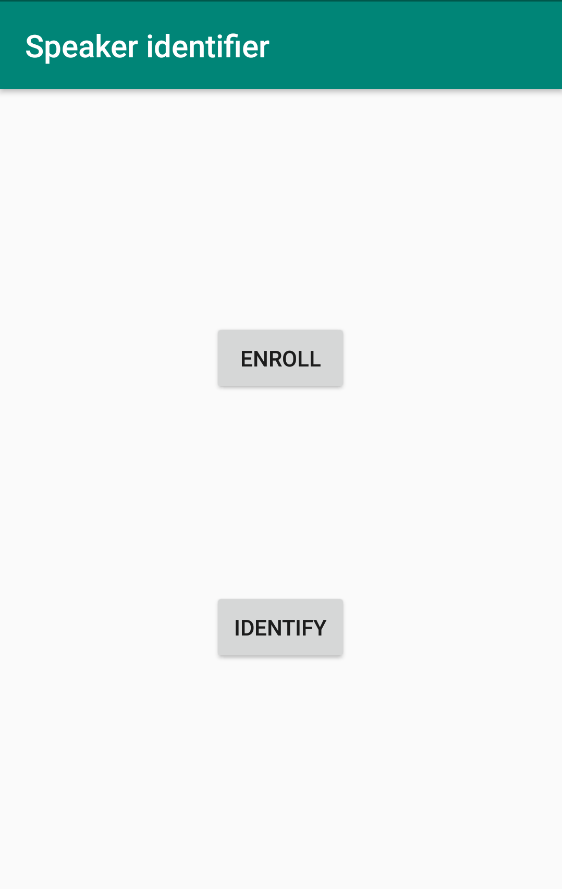
\includegraphics[width=40mm, keepaspectratio]{figures/app-main-screen.png}
	\caption{Menü.}
	\label{fig:app-main-screen}
\end{figure}
\ \\
A regisztrációs felületen megadjuk a nevet, majd a \emph{Record} gombra kattintva három másodperc múlva elindul a hangfelvétel, ami négy másodpercen keresztül tart. A felületen megjelenő információ folyamatosan tájékoztatja a felhasználót a hangfelvétel folyamatáról.

\begin{figure}[!ht]
	\centering
	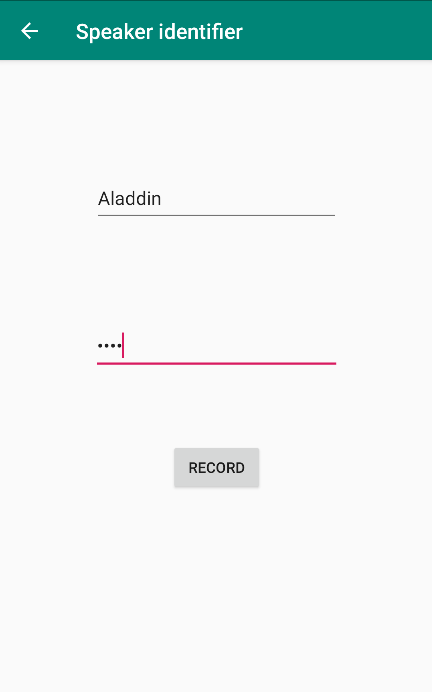
\includegraphics[width=40mm, keepaspectratio]{figures/app-register-screen-1.png}
	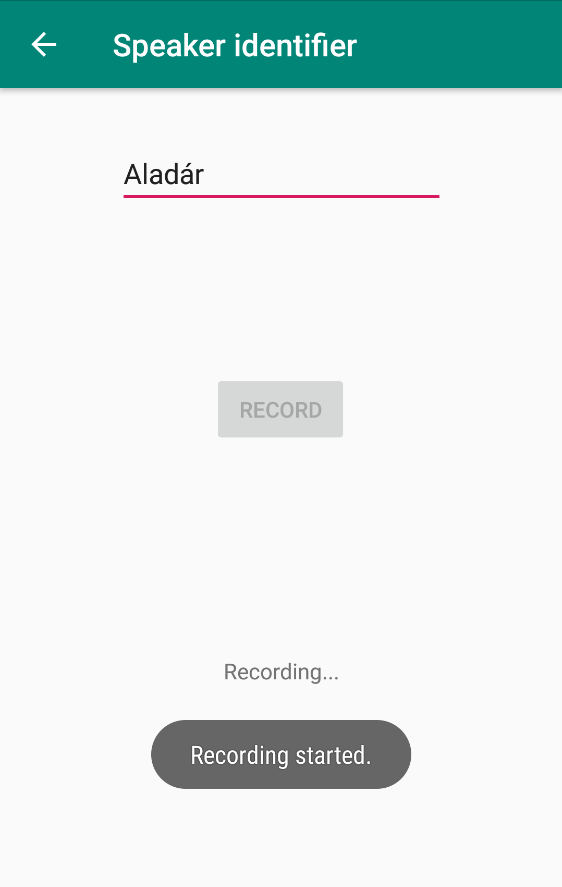
\includegraphics[width=40mm, keepaspectratio]{figures/app-register-screen-2.png}
	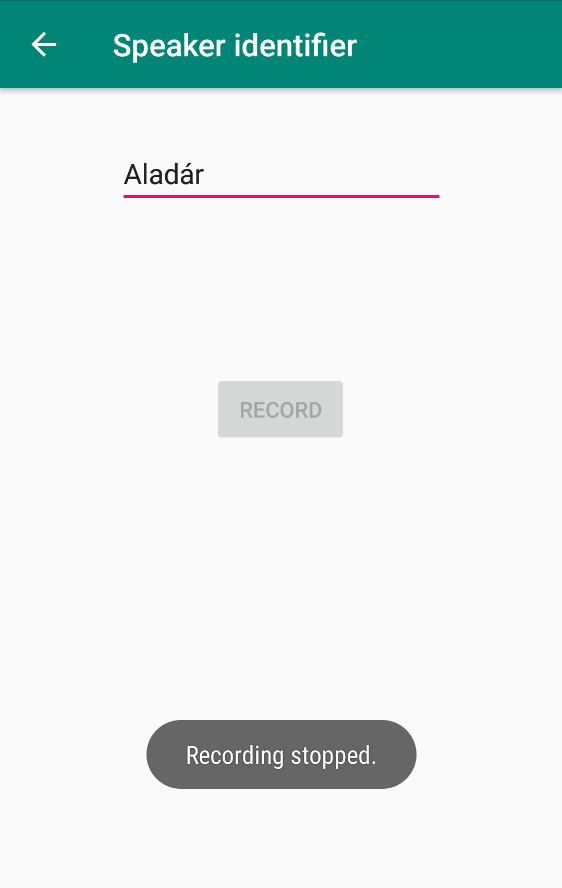
\includegraphics[width=40mm, keepaspectratio]{figures/app-register-screen-3.png}
	\caption{Felhasználói felület regisztrációhoz.}
	\label{fig:app-register-screen-1}
\end{figure}
\ \\
A zöld fejlécen a vissza nyílra kattintva visszajutunk a főmenübe. Ezt az opciót a manifest fájlban a \emph{parentActivityName} tag megadásával érhetjük el.

\begin{figure}[!ht]
	\centering
	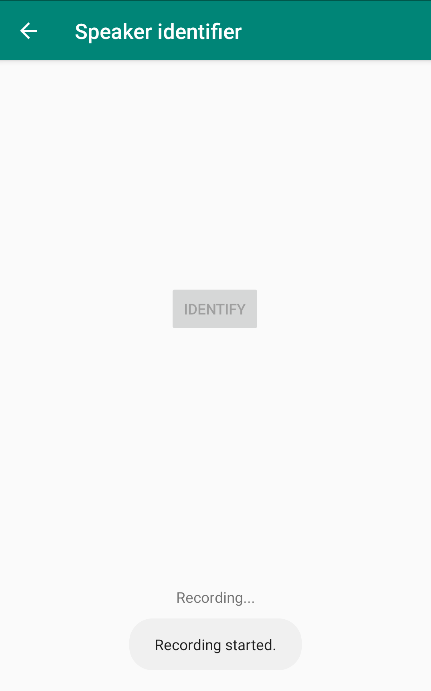
\includegraphics[width=40mm, keepaspectratio]{figures/app-identify-screen-1.png}
	\caption{Felhasználói felület azonosításhoz.}
	\label{fig:app-identify-screen-1}
\end{figure}

\newpage
A főmenüből az azonosító felületre lépve az \emph{Identify} gombra kattintva szintén visszaszámlálásra elindul a hangrögzítés, ami négy másodperig tart. Ezután megkapjuk a választ; az azonosított felhasználó nevét, vagy a nem sikerült azonosítani üzenetet.

\subsubsection{Osztálydiagram és részletes működés}

\begin{figure}[!ht]
	\centering
	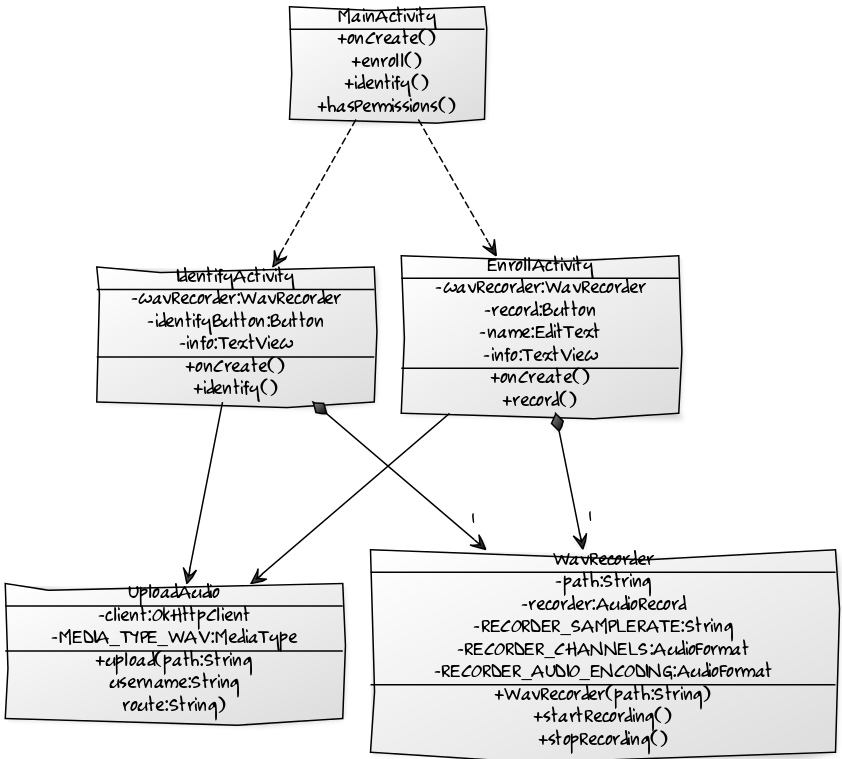
\includegraphics[width=130mm, keepaspectratio]{figures/app-class-diag.png}
	\caption{Beszélőfelismerő alkalmazás: Osztálydiagram.}
	\label{fig:app-class-diag}
\end{figure}

A \emph{MainActivity} osztály tartozik a főmenühöz. Amikor a főmenübe lépünk, az \emph{onCreate} metódus hívódik meg, amely ellenőrzi, hogy az alkalmazásnak megvannak-e a szükséges engedélyei a \emph{hasPermission} segédmetódus által. Ha igen akkor nem tesz semmit, egyébként a felhasználótól az összes engedély megadását kéri.
\newline
\newline
Az \emph{enroll} metódus a felületen az \emph{Enroll} gombhoz, az \emph{identify} az \emph{Identify} gombhoz tartozik. Mindkét függvény létrehoz egy-egy \emph{Intent}-et ami a hivatalos definíció szerint egy elvégzendő művelet absztrakt leírása. Az \emph{Intent} valójában arra jó, hogy egy felületről egy másik felületre lépjünk. A kiinduló felületen egy gombra kattintva (pl. \emph{Enroll}), a gombhoz tartozó listener metódus (\emph{enroll()}) hívódik meg, ami létrehoz egy \emph{Intentet} paraméterként átadva az elérni kívánt felülethez tartozó \emph{Activity} osztályt (\emph{EnrollActivity}). Ezután az \emph{Intentet} elindítva átlépünk a felületre.
\newline
\newline
A regisztrációs felületre lépve az \emph{onCreate} metódus meghívásakor az \emph{EnrollActivity} példányosít egy \emph{WavRecorder} objektumot a fájl elérési útjával paraméterezve. A \emph{record} metódus visszaszámlál, kiírja a felhasználónak az időzített üzeneteket, és elindítja majd megállítja a \emph{WavRecordert}.
\newline
\newline
Az időzítést az ajánlás szerint a \emph{Handler} osztály segítségével végeztem. Ennek előnye, hogy az időzített feladatokat egy háttérszálon futtatja, így nem blokkol. Így nem történhet meg, hogy egy hosszabb feladat elvégzése miatt a felületen nem kattinthatunk amíg az nincs kész.
\newline
\newline
Az \emph{IdentifyActivity} osztály nagyon hasonlóan működik. A különbség, hogy a \emph{EnrollActivity}-hez képest nem küld nevet és más címre küldi a hangfájlt.
\newline
\newline
Mindkét osztály a \emph{UploadAudio} objektumot használ a fájl szerverhez való elküldéséhez. Az \emph{UploadAudio} egy \emph{OkHttpClient} http klienst használ és \emph{multipart/form} Http POST kérést küld a szerver felé a hangfájllal ill. regisztrációkor a névvel. Ezután egy callback metódussal várja a szerver válaszát, amit az azonosító felületre továbbít.

\subsection{Szerver}

Szerver oldalon egy Flask webalkalmazás fut felhőben és REST API-val rendelkezik. Fogadja a klienstől érkező hangfájlokat, előfeldolgozza és tárolja őket. Azonosításkor a modellen prediktál, majd visszaküldi az eredményt a kliensnek.

\subsubsection{Flask}

A Flask egy Python nyelvhez készült web mikrokeretrendszer. Mikrokeretrendszernek nevezzük a minimális webalkalmazás keretrendszereket, amelyekből általában hiányoznak a autentikációs, autorizációs könyvtárak, az objektum-relációs leképzés stb.

A Flask két fő BSD-licencelt komponensre épül:

\begin{itemize}
	\item Werkzeug: A Werkzeug egy Python toolkit WSGI alkalmazásokhoz. Keretrendszereket lehet építeni rá és többféle Python verziót támogat. A WSGI egy hívási konvenció Pythonban írt webalkalmazásokhoz történő kérésekre.
	\item Jinja: Web template engine Python alkalmazásokhoz.
\end{itemize}
\ \\
A Flask előnye, hogy nagyon gyorsan és könnyedén lehet vele REST API-t készíteni és elindítani egy webalkalamzást. Nincs szükség más könyvtárakra, toolokra hozzá.
\newline
\newline
Képes egyszerre több kérést is kezelni. Külön sessionökből érkező kérések külön szálakon futnak, így a keretrendszer a szálkezelést is megoldja helyettünk. A következő fontosabb funkciókat biztosítja:

\begin{itemize}
	\item Webszerver fejlesztésre és debugger
	\item Unit tesztek integrált támogatása
	\item REST támogatása
	\item Jinja2 template weboldalakhoz
	\item WSGI 1.0 szabvány
	\item Jól dokumentált
\end{itemize}

\subsubsection{Projekt felépítése}

\begin{itemize}
	\item \emph{app}: A webalkalmazást indító és a logikát tartalmazó (előfeldolgozás, predikció, fájlok kezelése) illetve konfigurációt kezelő Python szkriptek könyvtára (app.py, preprocess.py).
	
	\begin{itemize}
		\item app/app.py
		\item app/model\_loader.py
		\item app/preprocess.py
		\item app/config.py
		\item app/paths.py
	\end{itemize}
	
	\item \emph{data}: Tartalmazza a klienstől regisztrációs fázisban kiszámolt vektorokat, az átlagolásra váró vektorokat és felhasználói adatokat.
	
	\begin{itemize}
		\item data/vectors: Az előfeldolgozott hangfájlok.
		\item data/vectors\_to\_average: Az átlagolásra váró, ideiglenesen tárolt vektorok helye.
		\item user\_dict: Felhasználó UID - felhasználónév összerendeléseket tartalmazó dictionary.
		\item passwords: Felhasználó UID - jelszó párokat tartalmazó dictionary.
	\end{itemize}
	
	\item \emph{model}: A beszélőfelismerésre használt modelleket tároló mappa.
\end{itemize}

\subsubsection{Részletes működés}

Az alkalmazás a következő REST végpontokat biztosítja a kliens számára:

\begin{itemize}
	\item /enroll: A regisztráció végpontja.
	\item /identify: Az azonosítási végpont.
	\item /authenticate: A jelszó alapú autentikáció végpontja.
\end{itemize}


\begin{figure}[!ht]
	\centering
	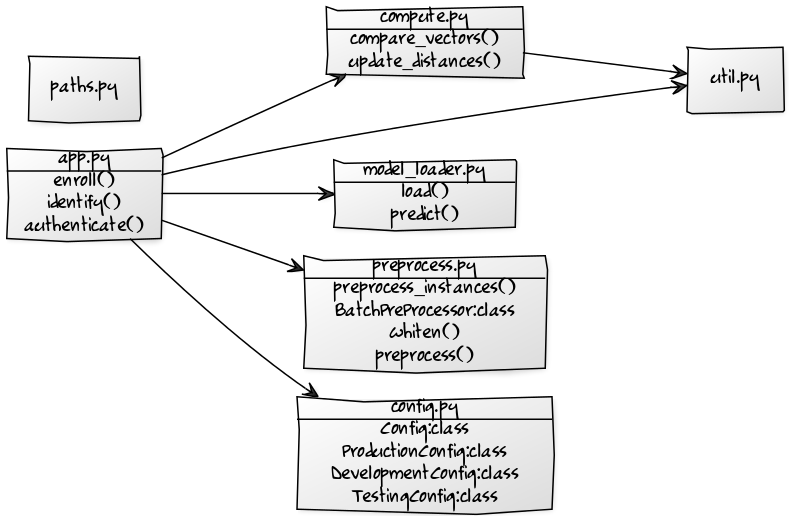
\includegraphics[width=130mm, keepaspectratio]{figures/flask-class-diag.png}
	\caption{Flask szerver: Osztálydiagram.}
	\label{fig:flask-class-diag}
\end{figure}

\begin{itemize}
	\item \emph{app.py}: Az \emph{app.py} implementálja a REST végpontokat. Az \emph{app.py} először létrehoz egy Flask objektumot, ezután betölti a megfelelő konfigurációt a \emph{config.py} szkriptben deklarált valamelyik objektummal. Betölti a modellt, majd elindítja az alkalmazást, ami a \emph{/enroll}, \emph{/identify} és \emph{/authenticate} útvonalakon \emph{HTTP POST} kérésekre vár.
	
	Mivel az alkalmazás egy prototípus és nincs szükség felhasználóspecifikus adatok tárolására néven és jelszón kívül, adatbázis helyett \emph{dictionary} tárolja az egyedi azonosító - felhasználónév illetve egyedi azonosító - jelszó párokat egy fájlba szerializálva, a hangvektorok pedig egyedi azonosítónévvel vannak eltárolva.
	
	\begin{itemize}
		\item \emph{enroll()}: Regisztrációkor megkapja a klienstől a hangmintát, a nevet és a jelszót. Amennyiben a hangminta nem támogatott formátumú, HTTP 400 (Bad Request) státuszkóddal válaszol. 
		\newline
		\newline
		Egyébként a felhasználónak létrehoz egy egyedi azonosítót és elmenti a jelszavát az \emph{passwords} dictionarybe. Preprocesszálja a hangmintát, a modell segítségével hangvektort készít belőle majd eltárolja. 
		\newline
		\newline
		A hangvektorok bináris formátumban kerülnek mentésre egyedi azonosító néven, így könnyen visszakereshetők.
		\newline
		\newline
		Végül frissíti a \emph{user\_dict} dictionaryt az aktuális felhasználó nevével és azonosítójával.
		\newline
		\item \emph{identify()}: A kliens ide küldi a hangmintát azonosításra. Amennyiben a hangminta nem támogatott formátumú, HTTP 400 (Bad Request) státuszkóddal válaszol. Ha a hangminta támogatott preprocesszálja, majd hangvektort készít belőle. Összehasonlítja a korábban regisztrált felhasználók hangvektorjaival, és megkeresi a minimális hasonlósági pontszámot. 
		\newline
		\newline
		Ha a minimális távolság meghaladja a biztonsági küszöböt, az aktuális vektort menti későbbi lehetséges átlagolás céljából. Ezután jelszó alapú autentikációs kérést küldd a kliensnek HTTP 403 (Forbidden) státuszkóddal. Mivel a HTTP protokoll állapotmentes, a kérés fejlécében elküldi a minimális távolsághoz tartozó felhasználó azonosítóját is az egyszerűség kedvéért (session kezelés helyett).
		\newline
		\newline
		Ha a minimális távolság a biztonsági küszöbön belül van, azaz az azonosítás sikeres volt, átlagolja az aktuális hangvektort az azonosítottal és HTTP 202 (Accepted) státuskóddal illetve a fejlécben az azonosított felhasználó nevével és egyedi azonosítójával válaszol.
		\newline
		\item \emph{authenticate()}: A \emph{/authenticate} végpontra küldött jelszó alapú autentikáció esetén hívódik meg. A klienstől érkező kérés tartalmazza az azonosítani kívánt felhasználó UID-t és a jelszót. Ellenőrzi, hogy a küldött jelszó megegyezik-e a korábban eltárolttal.
		\newline
		\newline
		Amennyiben igen, az autentikáció elején eltárolt hangvektort átlagolja a korábbival, majd HTTP 202 (Accepted) státuskóddal illetve a fejlécben az azonosított felhasználó nevével és egyedi azonosítójával válaszol.
		\newline
		\newline
		Ha a jelszavas autentikáció nem sikerült, törli az átlagolásra váró hangvektort és HTTP 403 (Forbidden) státuszkóddal válaszol a kliensnek.
	\end{itemize}

	\item \emph{model\_loader.py}:
		A fejlesztés kezdetén a modell betöltése a \emph{app.py}-ban volt implementálva. Mivel a Flask több szálat használ, problémát okozott, hogy a modellt valamelyik függvény hamarabb használta minthogy azt valóban betöltötte volna.
		\newline
		\newline
		Erre többféle megoldási lehetőség van. Például kötelezhetjük a Tensorflowt globális default gráf használatára. Mivel ez a megoldás csak részben működött, más javaslat alapján külön osztályba, a \emph{ModelLoader}be szerveztem. Ez az osztály felelős a modell betöltéséért illetve ez végzi el a predikciót.
		\newline	

	\begin{itemize}
		\item load(file\_name): Betölti az paraméterként kapott útvonalon található modellt.
		\item predict(model\_input, model): A bemenet és a választott modell alapján visszaadja a prediktált kimenetet.  
	\end{itemize}

		A \emph{ModelLoader} objektum inicializálásakor betölti a sziámi és a sima konvolúciós modellt is. Később a predict() függvényben paramétereiben állíthatjuk be, hogy melyik modellen szeretnénk a predikciót végrehajtani.
		
	\item \emph{preprocess.py}:
		
		\begin{itemize}
		\item \emph{whiten(batch, rms)}: A \emph{whiten} standardizálja a hangmintákat. Egy hangmintát egész számok sorozata reprezentál (PCM kódolás 4 vagy 16 biten). Először kivonja az átlagot minden számból, így a hangminta átlaga 0 lesz. Ezután újraskálázza a számokat, hogy ne legyenek kiugró amplitúdó értékek.
		\newline
		\item \emph{preprocess\_instances(downsampling, whitening)}: A \emph{preprocess} függvénynek két fő paramétere van: a hangminta hossza és a \emph{downsampling}, vagyis a csökkentett mintavételezési ráta. Ez a függvény végzi el a csökkentett mintavételezést és a standardizálást egy hangmintán.
		\newline
		\newline
		A csökkentett mintavételezés az eltérő mintavételi frekvencia miatt szükséges. Az Androidot futtató készülékek $8$ és $16$ bites PCM mellett $8$, $16$ és $44.1$ kHz-es mintavételi frekvenciákat támogatnak. Esetünkben a modellt $4$ kHz-en tanították a saját hangminták pedig $8$ kHz-esek ezért $2$-es csökkentett mintavételezés szükséges.
		\newline
		\item \emph{BatchPreProcessor(mode, instance\_preprocessor, target\_preprocessor)}: Ez az osztály wrapper funckiót lát el. Ez segít abban, hogy egységesen tudjuk kezelni az (inputs, outputs) klasszifikációs batcheket és a ([inputs\_1, inputs\_2], outputs) sziámi típusúakat is. A \emph{mode} paraméterrel megadjuk, hogy milyen típusú batchek előfeldolgozását szeretnénk. Az \emph{instance\_preprocessor} a bemenetek, a \emph{target\_preprocessor} a kimeneteket preprocesszáló függvény. Például \emph{BatchPreProcessor('classifier', preprocess\_instances(downsampling))}.
		\newline
		\item \emph{preprocess(audio\_file, sample\_length, downsampling)}: 
		Ez a függvény hatja végre a preprocesszálást. Beolvassa a paraméterként megadott hangmintát. A hangminta közepén \emph{sample\_length} hosszúságú darabot vág ki belőle. Létrehoz egy \emph{BatchPreProcessor} objektumot, előfeldolgozza a batchet, majd visszatér a feldolgozott hangmintával.
		\newline
		\newline
		Mivel a jelenleg használt modell $3$ másodperces és $4$ kHz-en mintavételezett hangmintákat vár a bemenetére, a saját $4$ másodperces hangmintákból $3$ másodperces darabokat vág ki a közepétől számolva $1,5$-$1,5$ másodperces távolságra. Erre azért van szükség, hogy ha a felhasználó kicsit később kezd el beszélni vagy hamarabb hagyja abba, a felvétel elején vagy végén lévő szünet ne kerüljön bele a mintába.
		\end{itemize}
\end{itemize}

\subsection{Fejlesztési környezet}

Ebben a fejezetben bemutatom a fejlesztéshez használt technológiai stacket. Szó lesz a szerver oldali és a kliens alkalmazáshoz használt toolokról, környezetekről.

\subsubsection{Git}

A Git egy nyílt forráskódú verziókezelő, ami a fejlesztésben rendkívül fontos. A verziókezelés nem csak akkor hasznos, ha többen dolgoznak egy projekten. Egyéni kódbázist
refaktorálás után ezáltal visszaállíthatunk, törölt fájlokat, kódrészleteket követhetünk vissza. A saját repositorymat GitHubon tároltam.

\subsubsection{Amazon EC2}

A webszerver a \ref{cloud_or_local} fejezet alapján Amazon EC2-es virtuális gépen fut. Az Amazon Elastic Compute Cloud szolgáltatás biztonságos és skálázható számítási kapacitást nyújt felhőben. Virtuális gépek bérelhetők rajta, amelyek utána testreszabhatók tárhely és erőforrások; processzor, memória szempontjából.
\newline
\newline
A felhasználók létrehozhatnak saját virtuális gépeket, amelyeken saját alkalmazásokat futtathatnak. Többféle fizetési modell közül választhatunk: Létezik óra vagy másodperc alapú, de saját dedikált gépet is bérelhetünk. Az AWS Educate segítségével diákok korlátozottan de ingyenesen használhatják az Amazon EC2 szolgáltatásokat egy megadott kreditszintig.
\newline
\newline
A virtuális gépen Ubuntu 16.04 operációs rendszer fut és ssh-n keresztül férhetünk hozzá. Ehhez a gép létrehozásakor lehet új kulcspárt generálni vagy meglévőket használni. A gép bootolásakor a publikus kulcs bekerül a \emph{~/.ssh/authorized\_keys} fájlba. Később ssh-nál a saját privát kulcsunkat megadva tudunk autentikálin. A virtuális menedzselése az AWS Console-on keresztül történik. A gépen futó Flask szerver portján engedélyezni kellett a be és kimenő forgalmat. Ehhez létre kell hozni egy új \emph{Security Groupot}, majd hozzáadni a megfelelő \emph{Rule}-t.
\newline
\newline
Az alkalmazás szempontjából nagy előny, hogy a felhőbeli gépet könnyen elérjük, és fejlesztés közben sem a saját gépünk erőforrásait használja. Hátránya, hogy a kényelmes remote fejlesztés több konfigurációt igényel.

\subsubsection{cmder}

A cmder egy Windowshoz készült konzol emulátor. Beépített Gittel és ssh-klienssel rendelkezik és több Linuxos parancsot is támogat. Használata sokkal kényelmesebb a Puttynál, könnyedén csatlakozhatunk vele a Linuxos géphez.
\newline
\newline
Az ssh klienst paraméterezni kell a privát kulcsunkkal és a timeout elkerülése érdekében saját ssh konfigurációs fájllal.
Eleinte probléma volt az ssh kapcsolat lejárási ideje, de ez kliens és szerveroldalon is könnyen konfigurálható. Linuxon a \emph{/etc/ssh/sshd\_config}-ban a \emph{ClientAliveInterval <seconds>} és \emph{ClientAliveCountMax <seconds>}, Windowson (jelen esetben kliens oldalon) a paraméterben megadott konfigurációs fájlban \emph{ServerAliveInterval <seconds>} és 
\emph{ServerAliveCountMax <seconds>} beállításokkal küszöbölhető ki.

\subsubsection{Anaconda}

Az Anaconda egy nyílt forráskódú Python és R disztribúció, amely több mint 1500 programcsomaggal, saját csomagkezelővel, grafikus felülettel és virtuális környezetkezelővel rendelkezik.

\begin{figure}[!ht]
	\centering
	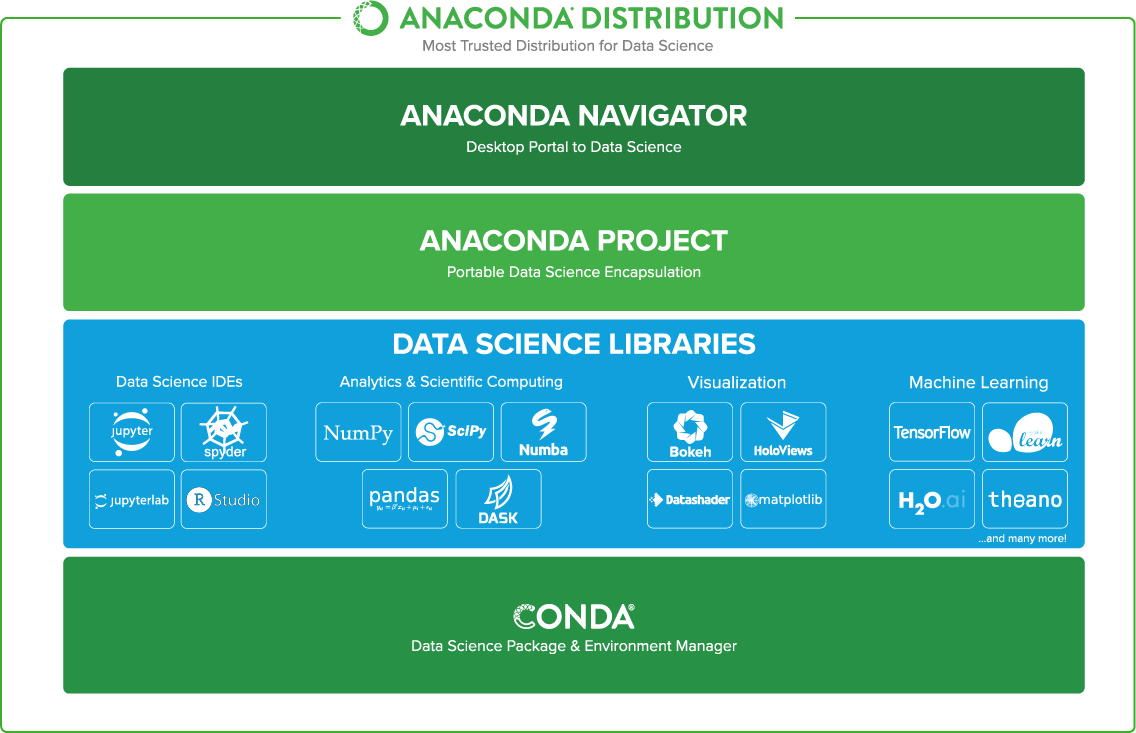
\includegraphics[width=150mm, keepaspectratio]{figures/anaconda-overview.png}
	\caption{Flask szerver: Osztálydiagram.}
	\label{fig:anaconda-overview}
\end{figure}
\ \\
Támogatja a gépi tanulást, tartalmazza a fontos gépi tanulási csomagokat (Keras, Tensorflow, Pytorch stb.), jupyter nootebookot. A virtuális környezetkezelővel a projekteknek külön virtuális környezetet hozhatunk létre. Ez fontos a verziók ütközésének elkerülése végett; Ha egy adott projektet Python 2.7-et használ, egy másik pedig Python 3.6-ot vagy ugyanolyan de eltérő verziójú programcsomagokat, akkor érdemes külön környezetet létrehozni nekik. A környezetek között a parancssorban navigálhatunk, csomagokat telepíthetünk rajtuk.
\newline
\newline
Az Anaconda Cloud további csomagokat, környezeteket, publikus és privát notebookokat tartalmaz. Ide feltölthetünk sajátot, illetve kereshetünk, telepíthetünk közülük csomagokat, környezeteket a saját gépünkre, környezetünkre.

\subsubsection{JetBrains PyCharm}

A JetBrain PyCharm egy Python programozási nyelvhez készült IDE. Azért esett erre a választás, mert van benne automatikus kódkiegészítés, intelligens kód navigáció - definícióra vagy használatra ugrás - és kód refaktorálás. Utóbbi a kód formázását és az importált csomagok rendezését jelenti.
\newline
\newline
Új projekt létrehozásakor saját virtuális környezetet hoz létre, de megadhatunk neki anaconda által létrehozottat, azt is képes kezelni. Jelen esetben a legfontosabb funkció a remote fejlesztés integrált támogatása volt.
\newline
\newline
A projekt beállításokban új Deployment létrehozásakor megadható a virtuális gép címe és a privát kulcs ssh-hoz. Megadhatók a lokális a remote mappák közötti mappingek és részletes szinkronizációs beállítások. A projekt interpreterének a remote gépen lévő Anaconda virtuális környezete által használt Python interpretert kell megadni, ez alapján a PyCharm feloldja a hozzá tartozó környezetet, látni fogja a programcsomagokat.
\newline
\newline
Szintén hasznos funckió a remote debugger, aminek segítségével a távoli virtuális gépen futó alkalmazást tudjuk debuggolni lokálisan.


\subsubsection{Android Studio}

A kliens oldali Android alkalmazás fejlesztéséhez Android Studiot használtam, ami az Android hivatalos fejlesztőkörnyezete. Az beépített templatek új \emph{Activity}k és a Layout Editor nagyban megkönnyíti a felhasználói felület fejlesztését. Támogatja emulátorok használatát, amelyeken debugolni is lehet.

\subsubsection{Genymotion}

Mivel az Android Studio emulátorai nem támogatják teljes mértékben az AMD processzorokat, külső emulátort használtam, a \emph{Genymotion}t. Ez egy külön alkalmazás és pluginnal csatlakoztatható az Android Studiohoz.

\section{Tesztelés és kiértékelés}

Az alkalmazást 8 emberrel teszteltem.

\section{Használati esetek és továbbfejlesztési lehetőségek}

Az implementált szoftver általános felhasználási módja a felhasználó azonosítás. Jelszó nélküli, csak hangalapú azonosítást kizárólag alacsony biztonsági szintű alkalmazásokban vagy funkciókban szabad használni. Minden komolyabb biztonságot követelő esetben vagy szigorú biztonsági küszöb, vagy kétfaktoros (hang és jelszó) autentikációt ajánlott használni.
\begin{itemize}
	\item 
\end{itemize}
